\documentclass[11pt,oneside,openany]{article}

\usepackage{graphicx}
\usepackage{color}    % to define macros for colors
\usepackage{listings} % package to include source code

\author{Matteo Franchin}

%TYPESETTING:----------------------------------------------------------

% Reset page margins properly for doublesided pages

% No headings
\pagestyle{plain}

% 1.5 interline spacing --> corresponds to linespread 1.3
% 2.0 interline spacing --> corresponds to linespread 1.6
\linespread{1.3}

\setlength{\marginparwidth}{0mm}
\setlength{\marginparsep}{0mm}
\setlength{\oddsidemargin}{0.7in} % corresponds to 1 + 0.7 = 1.7 inches
\setlength{\evensidemargin}{0.7in} % corresponds to 1.7 inches
\setlength{\textwidth}{145mm}
\setlength{\textheight}{220mm}
\setlength{\voffset}{-20mm}
\raggedbottom

%----------------------------------------------------------------------
% Extra colors

\definecolor{lightgrey}{cmyk}{0.05,0.05,0.05,0}
\definecolor{gray}{rgb}{0.5,0.5,0.5}

%----------------------------------------------------------------------
% Style for code listings

\lstdefinestyle{defaultstyle}{}
\lstset{language=Python}
\lstset{basicstyle=\ttfamily\scriptsize}
\lstset{showstringspaces=false}
\lstset{keywordstyle=\color{blue}}
\lstset{stringstyle=\color{red}}
\lstset{commentstyle=\color{gray}\emph}
\lstset{numbers=left,frame=single}
\lstset{backgroundcolor=\color{lightgrey}}

\newcommand{\vecs}[2]{\mathbf{#1_{\mathrm{#2}}}}

\begin{document}

\titlepage

\section{The Slonczewski Spin Transfer Torque in Nmag5}
In this document we explain how to use Nmag to create a simulation where
the applied field changes continuously with time.
This is an undocumented feature, which can be used, but for which a clean
user interface has not been defined, yet.
Defining a field which changes continuously in time can be useful for many
purposes: applying a pulse with optimal time dependency to excite spin waves
inside a system (with a well controlled window of frequencies) or extending
Nmag by adding an extra term to the applied field.
In this document we will show and explain one example which was used
in the course of the DYNAMAG project to compute the susceptibility
of a disk (spin waves where excited for a defined window of frequencies).
In this example, it is important to apply an homogeneous (in space) magnetic
field with a time dependecy which goes as
$\mathrm{sinc} \, \omega_{\mathrm{max}} t$,
as this allows exciting spin waves with freqencies from 0 to
$\omega_{\mathrm{max}}$.


\subsection{Example: dynamics of a disk excited by a sinc pulse}
In this example we consider a disk. We create the mesh using Netgen and
the following geometry specification file:
%
%\lstinputlisting{disk.geo}
%
The resulting mesh is shown in Fig. \ref{fig:mesh}.
%
\begin{figure}[h]
\begin{center}
%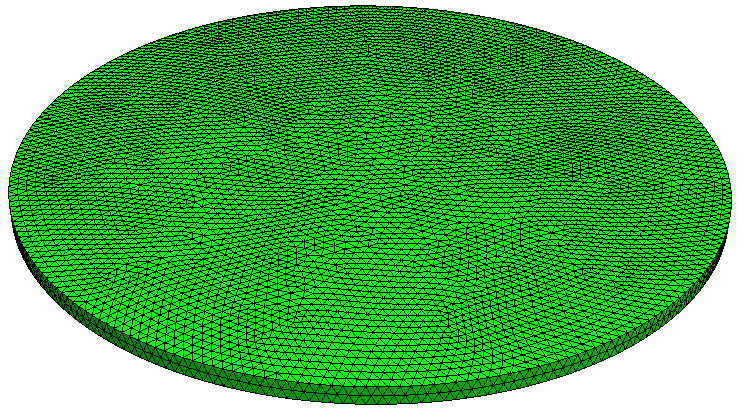
\includegraphics[width=10.0cm]{disk}
\caption[Sketch]{A picture of the mesh used in the simulation.}
\label{fig:mesh}
\end{center}
\end{figure}
%
The simulation script is split in the two figures Fig. \ref{fig:script1of2} and
\ref{fig:script2of2}.  The script can be used to perform two simulations: if
the script is ran for the first time, it just perform a relaxation and saves
the relaxed magnetisation to a file with name \verb|relaxed.h5|. If the script
is ran for a second time, it checks whether this file exist, it finds it, and
loads the initial magnetisation from it. It then applies a pulsed magnetic
field and records the dynamics to disk.

\begin{figure}[!p]
\lstinputlisting[linerange=1-39]{../../slonczewski/validation/nmag/run.py}
\caption{Part 1.}
\label{fig:script1of2}
\end{figure}

\begin{figure}[!h]
\lstinputlisting[linerange=40-60,firstnumber=40]{../../slonczewski/validation/nmag/run.py}
\caption{Part 2.}
\label{fig:script2of2}
\end{figure}

We will now describe the script line-by-line:

\textbf{Lines 1-6:} these are the usual import statements, which often occur
in Nmag scripts. Notice the nmag5 specific imports (\verb|from nmag.nmag5 ...|
and \verb|from nsim.model ...|).

\textbf{Lines 7-12:} these lines define some useful variables such as
\verb|ps| for picosecond, \verb|nm| for nanometre.  The also define the
spherical angles for the polarisation direction \verb|theta| and \verb|phi|,
the size of the mesh, the applied current density and the applied field
(in milli-Tesla).

\textbf{Lines 13-21:} if the mesh \verb|film.nmesh.h5| does not exist, then
we create it, by using the \verb|netgen_mesh_from_string| function from the
\verb|nsim.netgen| module. Note that we provide the geo file as a Python
string. The function does automatically invoke Netgen (which must be installed
on the system) and does convert automatically the Neutral output to the
Nsim \verb|nmesh.h5| file format.

\textbf{Lines 22-30:} the material is defined, together with its anisotropy
parameters.

\textbf{Lines 31-34:} Other three STT-related parameters are defined for the
material. Notice that here the interface is not polished and the material
parameters are added just as attributes of the material \verb|mat|. (we should
repair this, either by adding these extra parameters to the \verb|MagMaterial|
class or by accepting a \verb|**kwargs| in \verb|MagMaterial|.

\textbf{Lines 35-38:} the function \verb|setup_simulation| is used to create
the materials, create the simulation object and load the mesh. These operations
are collected together in this function, as they are needed twice: once for the
relaxation simulation and a second time for the dynamics simulation.  Notice,
how the tolerances are set. Controlling all the tolerances is very important in
this kind of simulations, where accuracy can substantially improve the
results. The function \verb|setup_simulation| returns the simulation object, so
it can be further manipulated after the function has been called.

\textbf{Lines 39-50:} Other STT-related quantities are set. In particular,
the direction of the polarisation \verb|P_direction| is computed from the
polar angles and it is used to set the vector \verb|sl_fix|.
The value of the current density is also set. 

\textbf{Lines 51-57:} The tolerances for the simulation are set
and the relaxation is launched, saving the averages every 5 picoseconds.
Notice that the stopping criterion is disabled (\verb|stopping_dm_dt| is set
to zero) and the simulation is forced to quit after 10 nanoseconds
(\verb|do=[("exit", at("time", 10000*ps))])|).
Notice also that the method \verb|Simulation.set_params| is capable
of setting the demag tolerances \verb|demag_..._tol| and the preconditioner
tolerances \verb|ts_pc_..._tol|. This is a new feature of Nmag5 (and is
not yet available in Nmag4, where one needs to provide these tolerances
in a dictionary passed to the \verb|Simulation| object during creation,
which also means that one cannot change them later on in the simulation).


%
%\lstinputlisting[linerange=87-87,firstnumber=87]{script.py}
%

\subsection{Final remarks}
This script can also be used as a model for computing dispersion relations.
Typically one would then use the mesh of a wire.  He would also use a pulse
which is not homogeneous in space, but has rather a sinc dependency along the
direction of the propagation of the spin waves. This requires little
modifications: it is just enough to redefine the variable \verb|pulse| (which
was set to the value \verb|[0.0, 0.0, 1.0]| in the script) as a function
(\verb|def pulse(r): ...|).

\end{document}
